%-----------------------------------------------------------------------------%
\chapter{LANDASAN TEORI}
%-----------------------------------------------------------------------------%

%
\vspace{4.5pt}

\begin{flushleft}
    \begin{justify}
        \section{Tinjauan Pustaka}
    Banyak penelitian sebelumnya yang berkaitan dengan pengembangan, perancangan, dan pembuatan sebuah aplikasi menggunakan
    \textit{Systems Development Life Cycle} (SDLC) \textit{Rapid Application Development} (RAD). Dalam penelitian yang dikerjakan oleh
    Meidyan Permata Putri dan Hendra Effendi \cite{web waterfall} dihasilkan kesimpulan bahwa penerapan metode RAD sudah dapat memberikan hasil maksimal ditunjukkan dengan sistem yang dibuat
    dapat memenuhi kebutuhan pengguna. Dalam penelitian yang dikerjakan oleh Abdul Rahman \cite{jurnal RAD UAT} dihasilkan kesimpulan bahwa pembuatan aplikasi pembelajaran daring dengan menggunakan metode RAD bisa diterima dengan baik oleh pengguna dengan presentase sebesar 91\% dengan pengujian \textit{User Acceptance Testing} (UAT).
    Dalam penelitian yang dikerjakan oleh Diah Aryani, Malabay, dan Hani Dewi Ariessanti [] dihasilkan kesimpulan bahwa penggunaan RAD dapat memudahkan pihak terkait dalam melakukan penelusuran dan pengelolaan umpan balik dari kuesioner dan
    pengujian UAT menghasilkan 2 nilai yaitu 91\% dari pihak kemahasiswaan dan 88\% dari pihak mahasiswa.

    \vspace{1cm}
    \section{Dasar Teori}

        \subsection{\textit{Monitoring} dan Kontrol}
        Menurut Dr. Harry Hikmat (2010), monitoring adalah proses pengumpulan
        dan analisis informasi berdasarkan indikator yang ditetapkan secara sistematis dan
        berkelanjutan tentang kegiatan/program sehingga dapat dilakukan tindakan
        koreksi untuk penyempurnaan program/kegiatan itu selanjutnya
        Sistem kontrol atau
        sistem kendali adalah kumpulan dari beberapa komponen yang terhubung satu
        sama lainnya, sehingga membentuk suatu tujuan tertentu yaitu mengendalikan
        atau mengatur suatu sistem (Ogata, 1997). 
        \\

        \subsection{Aplikasi \textit{Mobile}}
        Aplikasi \textit{mobile} adalah program perangkat lunak yang dirancang untuk dijalankan di smartphone, tablet, dan perangkat lain \cite{mobile}. Urgensi penggunaan Aplikasi yang dikembangkan berbasis mobile adalah semakin meningkatnya pengguna smartphone yang membutuhkan berbagai macam alat sebagai fasilitator dalam kegiatan sehari-hari. Sebagai fasilitator, aplikasi mobile harus mampu menyediakan informasi agar dapat menjadi sumber data bagi penggunanya dan mampu meningkatkan produktifitas pengguna. 
        \\
        \subsection{\textit{Rapid Application Development} (RAD)}
        Dalam referensi \cite{Sukamto} terdapat lima tahapan dalam model RAD : (1) Pemodelan bisnis, (2) Pemodelan data, (3) Pemodelan proses, (4) Pembentukan aplikasi, (5) Pengujian dan \textit{turnover} .
        
        \begin{figure}[ht]
            \centering
           
	    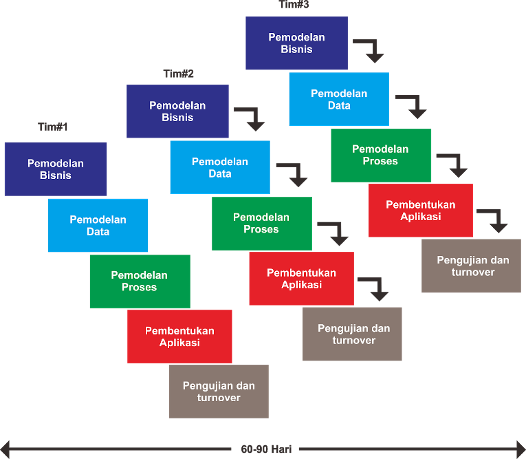
\includegraphics[width=6cm]{images/RAD.png}\\
            \caption{Gambar Ilustrasi Model RAD}
        \end{figure}
        \vspace{8cm}
        Berdasarkan Gambar 3, dapat diperhatikan penjabaran sebagai berikut :
        \begin{enumerate}[label=\alph*.]
            \item Pemodelan Bisnis\\
            Pada tahap ini output yang dihasilkan berupa dokumen \textit{Software Requirements Specification} (SRS) yang meliputi informasi ketentuan aplikasi yang akan dibuat. Dokumen tersebut mencakup informasi apa saja yang harus dibuat, siapa yang harus membuat informasi itu, bagaimana alur informasi itu, proses apa saja yang terkait informasi itu.
            \item Pemodelan Data\\
            Memodelkan data apa saja yang dibutuhkan berdasarkan pemodelan bisnis dan mendefinisikan atribut-atributnya beserta relasinya dengan data-data yang lain. 
            \item Pemodelan Proses\\
            Mengimplementasikan fungsi bisnis yang sudah didefinisikan terkait dengan pendefinisian data. 
            \item Pembuatan Aplikasi\\
            Mengimplementasikan pemodelan proses dan data menjadi program. Model RAD sangat menganjurkan pemakaian komponen yang sudah ada jika dimungkinkan.
            \item Pengujian dan Pergantian\\
            Menguji komponen-komponen yang dibuat. Jika sudah teruji maka tim pengembang komponen dapat beranjak untuk mengembangkan komponen berikutnya.\\
        \end{enumerate}

        \subsection{Flutter}
        Flutter merupakan sebuah framework aplikasi mobile yang bersifat open source (terbuka) yang diciptakan oleh Google. Flutter dapat digunakan dalam pengembangan aplikasi mobile untuk sistem operasi Android dan iOS, bahkan juga dapat digunakan dalam pengembangan Web ataupun Desktop dari codebase tunggal. Flutter merupakan framework dengan penggunaan Bahasa Dart.
Berikut ini bebrapa kelebihan dari Flutter \cite{flutter} :
\begin{enumerate}
    \item \textit{Package modules} sudah terkoneksi secara otomatis di dalam flutter, sehingga tidak terlalu repot untuk memanggil secara manual melalui terminal
    \item Dart menggunakan konsep OOP (\textit{Object Orinented Programming})
    \item \textit{Setup} secara manual jauh lebih mudah, apabila kita memerlukan \textit{library} baru, cukup tambahkan di bagian puspec.yaml
    \item Performa cepat dan  \textit{smooth}
    \item Data management menggunakan state sehingga lebih mudah dalam penggunaannya
    \item Adanya fitur \textit{Hot Reload} yang membantu debug lebih cepat
    \item Disupport oleh IDE yang sudah familiar dikalangan developer android, seperti Android Studio dan Visual Code\\
    
\end{enumerate}


        \subsection{\textit{Application Programming Interface} (API)}
            \textit{Application Programming Interface} atau API memungkinkan sebuah perusahaan untuk membuka data dan fungsionalitas aplikasi kepada \textit{developer} pihak ketiga / eksternal, mitra bisnis, dan departemen internal di dalam perusahaan tersebut. 
            Hal ini memungkinkan layanan dan produk untuk berkomunikasi satu sama lain dan memanfaatkan data dan fungsionalitas satu sama lain melalui \textit{interface} yang terdokumentasi. 
            \textit{Developer} tidak perlu tahu bagaimana API diimplementasikan; \textit{developer} hanya menggunakan \textit{interface} untuk berkomunikasi dengan produk dan layanan lain. 
            Penggunaan API telah melonjak selama dekade terakhir, sampai pada tingkat di mana banyak aplikasi web paling populer saat ini tidak akan mungkin tanpa API \cite{API}. Secara tradisional, API merujuk ke \textit{interface} yang terhubung ke aplikasi yang mungkin telah dibuat dengan salah satu bahasa pemrograman tingkat rendah, seperti Javascript. API modern mematuhi prinsip REST dan format JSON dan biasanya dibuat untuk HTTP, menghasilkan \textit{interface} yang ramah kepada \textit{developer} yang mudah diakses dan dipahami secara luas oleh aplikasi yang ditulis dalam Java, Ruby, Python, dan banyak bahasa lainnya.
            \\


        \subsection{\textit{Database}}
        \textit{Database} adalah \textit{collection} dari informasi terstruktur yang terorganisir atau data, biasanya disimpan secara elektronik dalam sistem komputer \cite{Database}. Sebuah \textit{database} biasanya dikendalikan oleh \textit{Database Management System} (DBMS). Data dan DBMS bersama dengan aplikasi yang terkait dengannya disebut sebagai sistem basis data atau sering disingkat menjadi basis data saja.
        Data dalam tipe \textit{database} yang paling umum yang beroperasi saat ini biasanya dimodelkan sebagai baris dan kolom dalam serangkaian tabel untuk membuat pemrosesan dan kueri data menjadi efisien. Data kemudian dapat dengan mudah diakses, dikelola, dimodifikasi, diperbarui, dikendalikan, dan diatur. Sebagian besar \textit{database} menggunakan \textit{structured query language} (SQL) untuk menulis dan mengolah data. 
        Salah satu SQL yang sering digunakan adalah MySQL yang merupakan sistem manajemen basis data relasional yang tersedia \textit{open source} sehingga memudahkan pengguna.
        \\
        \subsection{\textit{Flowchart}}
        \textit{Flowchart} sering juga disebut dengan \textit{process flowchart, process flow diagram} atau diagram alir. Flowchart adalah gambaran langkah-langkah terpisah dari suatu proses secara berurutan. 
        \textit{Flowchart} sangat umum digunakan dan dapat diadaptasi untuk berbagai tujuan, dapat digunakan untuk menggambarkan berbagai proses, seperti proses manufaktur, proses administrasi/layanan, atau gambaran rencana proyek \cite{Flowchart}.
        Beberapa kondisi yang disarankan untuk menggunakan \textit{flowchart} yaitu 
        (1) Untuk membangun pemahaman tentang bagaimana suatu proses dilakukan,
        (2) Untuk mempelajari proses guna melakukan perbaikan,
        (3) Untuk mengomunikasikan kepada orang lain bagaimana suatu proses dilakukan,
        (4) Ketika komunikasi yang lebih baik diperlukan antara orang-orang yang terlibat dengan proses yang sama,
        (5) Untuk mendokumentasikan sebuah proses saat perencanaan proyek
        \\\\

        \subsection{\textit{Use Case} Diagram}

        \subsection{\textit{Black Box Testing}}

        \subsection{\textit{User Acceptance Testing} (UAT)}
        \noindent User Acceptance Testing (UAT) adalah pengujian terakhir yang dilakukan oleh user secara langsung, dan pada saat pengujian berlangsung pembuatan dokumen juga dilakukan sebagai bukti penerimaan sistem oleh pengguna. 
        \textcolor{red}{[Mutiara, A. B., Awaludin, R., Muslim, A. and T. Oswari, “Testing Implementasi Website Rekam Medis Elektronik Opeltgunasys Dengan Metode Acceptance Testing,” 2014.].
        }
        

        \subsection{Skala \textit{Likert}}






    \end{justify}
    



\end{flushleft}



\newpage